\chapter{Introduzione al Machine Learning}

\section{Prime definizioni di Machine Learning}

\subsection{Arthur Samuel - 1959}

Nel 1959, Arthur Samuel fornisce una \textbf{definizione di machine learning}: il machine learning \`e il campo di studi che abilita i computer ad \textbf{imparare}, \textbf{senza essere esplicitamente programmati}.

Il paradigma alla base \`e fortemente diverso da quello tipico: se un algoritmo classico \`e \textbf{programmato ad hoc} per risolvere un task e si comporta in maniera prettamente \textbf{deterministica}, un algoritmo di machine learning pu\`o \textbf{imparare a risolvere problemi} associati a vasti insiemi di dati (classificare elementi, riconoscerli, trovare correlazioni). Questo permette di spostare il focus: non pi\`u sullo sviluppo di tutti gli step necessari affinch\'e un algoritmo risolva \textbf{un problema specifico}, ma sulla creazione di un modello che riesca ad apprendere come risolvere \textbf{un insieme di problemi simili}.

\subsection{Perch\'e abbiamo bisogno del Machine Learning}

L'approccio utilizzato finora per risolvere i problemi \`e quello di:

\begin{itemize}
\item Trovare una logica per risolvere il problema.
\item Scrivere un programma.
\item Suddividerlo in pezzi pi\`u piccoli (funzioni).
\item Automatizzare l'approccio.
\end{itemize}

Questo funziona bene per problemi di natura fortemente univoca, che sappiamo come risolvere, ad esempio:

\begin{itemize}
    \item Computare l'area di un poligono.
    \item Risolvere equazioni differenziali.
\end{itemize}

Nel caso del poligono, supponendo di voler calcolare l'area di un rombo, i dati presi in input sarebbero dati dalla coppia $(x_1, x_2)$, contenente le lunghezze della diagonale principale e secondaria. Questi dati, passati ad un algoritmo, permettono di calcolarne l'area $\frac{x_1 x_2}{2}$ e generarne un output:

$$
\text{Dati} \to \text{Programma che risolve un task} \to \text{Output}.
$$

Alcuni problemi tuttavia presentano un alto grado di \textbf{incertezza}, che li rende pi\`u difficili da affrontare. Non poter fare assunzioni sui dati in input, e non conoscere tutti i possibili task, rende impossibile l'utilizzo di algoritmi standard per compiti del tipo:

\begin{itemize}
\item Classificazione di email spam e non spam.
\item Object detection.
\end{itemize}

Il machine learning rappresenta la soluzione ideale a problemi di questo tipo, proponendo una nuova pipeline:

$$
\text{Dati + Output atteso} \to \text{Machine Learning} \to \text{Soluzioni su nuovi dati}.
$$

\subsection{Esempio delle email spam e non-spam}

Vogliamo creare un algoritmo di machine learning in grado di determinare se una mail \`e spam o meno. Il nostro obiettivo \`e quindi classificare ciascuna di queste come \textbf{spam}, o \textbf{ham}\footnote{Email legittima, non spam.}.

\begin{itemize}
    \item \verb|Compra prodotto a 10$! Offerta imperdibile! |$\rightarrow$ Spam
    \item \verb|Ciao Giovanni, come stai?| $\rightarrow$ Ham
\end{itemize}

\subsection{Tom Mitchell - 1998}

Un algoritmo \textbf{apprende dall'esperienza} $E$ rispetto a una certa classe di \textbf{task} $T$ e a una misura di \textbf{performance} $P$. Se la sua \textbf{performance} nel compito $T$, misurata tramite $P$, migliora con l'\textbf{esperienza} $E$, allora quel modello ha appreso con successo.

\section{Definizioni fondamentali}

\subsection{Definizione di Task}

Il \textbf{task} rappresenta il problema che deve essere risolto. Nell'esempio di determinare se una mail \`e spam o meno, il task \`e quello di \textbf{predire} l'etichetta ($Y=\text{``spam''}$ oppure $Y=\text{``ham''}$), ed \`e strettamente legato al modello, che rappresentiamo come funzione parametrizzata, indicata con $h_\theta$.

\subsection{Definizione di Esperienza}

\begin{quote}
L'esperienza si definisce come l'insieme di informazioni a cui il modello \`e esposto durante il processo di apprendimento e a partire dalle quali aggiorna (ossia modifica) i propri parametri interni.
\end{quote}

\paragraph{Supervised learning.}
Nel \textbf{supervised learning}, l'esperienza \`e un dataset di esempi osservati, cio\`e un insieme di \emph{realizzazioni} delle variabili aleatorie $(X, Y)$. Denotiamo il dataset con:
\[
D = \{(x^{(i)}, y^{(i)})\}_{i=1}^m,
\]
dove $x^{(i)}$ e $y^{(i)}$ sono rispettivamente input e output osservati per l'esempio $i$-esimo. In genere si assume che gli esempi siano estratti in modo i.i.d.\ da una distribuzione incognita $\mathcal{D}$.

\paragraph{Reinforcement learning.}
Nel \textbf{reinforcement learning}, l'esperienza assume una forma pi\`u generale: essa coincide con qualunque interazione che il modello ha con l'ambiente. Ad esempio, se il modello sta cercando di uscire da un labirinto, la sua esperienza al tempo $t$ pu\`o essere rappresentata dalla tupla:
\[
E_t = (S_t, A_t, R_t, S_{t+1}),
\]
dove $S_t$ corrisponde allo stato attuale in cui si trova il modello, $A_t$ all'azione intrapresa dato lo stato corrente, $R_t$ alla ricompensa ricevuta a seguito dell'azione e $S_{t+1}$ allo stato successivo.

\medskip
\noindent
\textit{In sintesi: l'esperienza \`e l'informazione (storico dei dati oppure interazioni con l'ambiente) a cui il modello \`e esposto e da cui impara, cio\`e tramite cui modifica i suoi parametri interni.}

\subsection{Definizione di Performance}

La misura di performance $P$ valuta quanto bene il modello risolve un task $T$. In alcuni casi $P$ \`e una metrica da \textbf{massimizzare} (per esempio l'accuracy, con valori in $[0,1]$), mentre in altri casi \`e pi\`u naturale definire una \textbf{loss} $\ell$ da \textbf{minimizzare} (per esempio il mean squared error, con valori in $[0,+\infty)$).

Supponiamo che il nostro algoritmo abbia previsto un insieme di etichette per un dato numero di email che indichiamo con:
\[
\{\hat{y}_i\}.
\]
\noindent
Dove il simbolo ``hat'' indica che il dato non \`e stato osservato ma \textbf{previsto}. L'insieme delle etichette corrette \`e invece dato da
\[
\{y_i\}.
\]
\noindent
Per valutare la qualit\`a del metodo, possiamo confrontare i due insiemi con una misura di performance:
\[
P(\{y_i\}, \{\hat{y}_i\}).
\]
\noindent
Se $P$ \`e normalizzata (come l'accuracy), possiamo interpretare $1-P$ come errore (\emph{error rate}). In generale, per definire l'errore si usa una loss $\ell$.

\subsection{Esempio completo}

Siano:
\begin{itemize}
\item $x^{(1)}$: Il testo dell'email 1: ``Compra prodotto a 10\$! Offerta imperdibile!''
\item $x^{(2)}$: Il testo dell'email 2: ``Ciao Giovanni, come stai?''
\item $y^{(1)}$: L'etichetta \textbf{spam}
\item $y^{(2)}$: L'etichetta \textbf{ham}
\item $h_\theta$: Il modello
\end{itemize}

\noindent
Allora
\[
h_\theta(x^{(1)}) = \hat{y}^{(1)}
\qquad \text{e} \qquad
h_\theta(x^{(2)}) = \hat{y}^{(2)}.
\]

\section{Task, esempi ed etichette}

Un esempio (o osservazione) \`e una raccolta di valori misurati. Un esempio \`e rappresentato da un vettore:
\[
x \in \mathbb{R}^{d},
\]
scritto anche come:
\[
x = (x_1, x_2, \dots, x_d).
\]

I valori del vettore $x$ sono detti \textbf{features}, in quanto rappresentano \textbf{attributi misurabili} (o una rappresentazione numerica) dell'input. Se la dimensionalit\`a di $x$ \`e $d$, diremo che l'esempio ha $d$ features. Nella maggior parte dei casi, ogni esempio $x$ \`e abbinato a un output desiderato $y$, detto \textbf{etichetta}. Un task \`e quindi un modo di elaborare un input $x$ per ottenere un output $y$.

Torniamo al nostro esempio: determinare se un'e-mail \`e spam o ham. In questo caso, l'input \`e l'e-mail; le features possono essere caratteristiche dell'e-mail, come il numero di errori ortografici o la presenza di alcune parole chiave; l'output atteso \`e l'etichetta (spam o ham).

\section{Features}

\subsection{Estrazione}

Per gestire le e-mail, dobbiamo prima trasformarle in un'\textbf{entit\`a quantificabile}. Questo di solito viene fatto \textbf{identificando alcune caratteristiche} dei dati che sono \textbf{rilevanti per il compito dato} (numero di errori ortografici o presenza di alcune parole chiave). In pratica, stiamo cercando una funzione $f$ che trasformi l'entit\`a dalla sua forma originale a una forma di destinazione, adatta a risolvere un compito specifico:
\[
x \rightsquigarrow f(x) \rightsquigarrow \overline{x}.
\]
Dove $x$ \`e il dato grezzo di input (ad esempio, il messaggio di posta elettronica completo), $f$ \`e la funzione di trasformazione e $\overline{x}$\footnote{Su questa notazione: da ora in poi, quando ci riferiremo all'output della trasformazione, non useremo pi\`u $\overline{x}$, ma direttamente $x$, dando per scontato il passaggio di rappresentazione $f(x)$.} \`e l'output della trasformazione, che sar\`a l'input dell'algoritmo di apprendimento automatico.

La funzione $f$ \`e chiamata \emph{rappresentazione}. L'output della trasformazione \`e anch'esso chiamato rappresentazione. Poich\'e rappresentando i dati otteniamo un vettore di features, il processo di rappresentazione dei dati \`e talvolta chiamato \textbf{feature extraction}. Non esistono ``rappresentazioni universali'', ma solo rappresentazioni utili a un determinato compito.

\noindent
Le rappresentazioni sono di due tipi:
\begin{itemize}
\item Create a mano.
\item Apprese.
\end{itemize}

\noindent
L'estrazione delle features \textbf{mette in luce caratteristiche salienti} trascurandone altre.

\subsection{Definizione formale}

Generalmente, l'output di una funzione di rappresentazione \`e nella forma:
\[
x = (x_1, x_2, \dots, x_d), \quad x \in \mathbb{R}^d.
\]

\noindent
Questo \`e composto da un insieme di features. \textbf{Una feature \`e la specifica di un attributo misurabile} dell'input: una quantit\`a che rappresenta \textbf{aspetti dei dati} utili per risolvere il problema considerato. Ad esempio, il colore pu\`o essere un attributo; ``il colore \`e blu'' \`e una feature estratta da un esempio.

\noindent
Le features possono essere di due tipi principali:
\begin{description}
    \item[Categoriche:] un numero finito di valori discreti. Questi possono essere:
    \begin{itemize}
        \item \textbf{Nominali:} non esiste \textbf{alcun ordinamento} tra i valori (es.\ cognomi, colori).
        \item \textbf{Ordinali:} esiste un \textbf{ordinamento rilevante} (es.\ basso, medio, alto).
    \end{itemize}
    \item[Continue:] comunemente un \textbf{sottoinsieme di numeri reali}, dove i valori sono ordinati e confrontabili. I numeri interi sono solitamente trattati come continui nei problemi pratici.
\end{description}

\section{Esempio delle Email Spam e Non Spam}

Consideriamo il nostro esempio in cui vogliamo distinguere le e-mail spam da quelle non spam. L'input del processo sono i messaggi di posta elettronica, quindi dobbiamo trasformarli in vettori di features:
\[
x = (x_1, x_2, \dots, x_d),
\]
con un processo di \emph{feature extraction}.

Naturalmente, ci aspettiamo che le features estratte siano \textbf{utili per risolvere il nostro compito} di determinare se un'e-mail \`e spam o ham. Possiamo notare che le e-mail di spam spesso includono errori ortografici e parole come ``Acquista'', ``occasione'' e ``10\$''. Quindi, potremmo decidere di rappresentare ogni messaggio di posta elettronica con due numeri (cio\`e $d=2$):
\begin{itemize}
    \item Il conteggio degli errori ortografici.
    \item Il numero di volte in cui alcune parole o pattern specifici appaiono nel testo.
\end{itemize}

Una volta che i messaggi di input sono stati convertiti in \textbf{vettori di features}, possono essere visti come \textbf{vettori nello spazio} $\mathbb{R}^2$.

\begin{figure}[htbp]
    \centering
    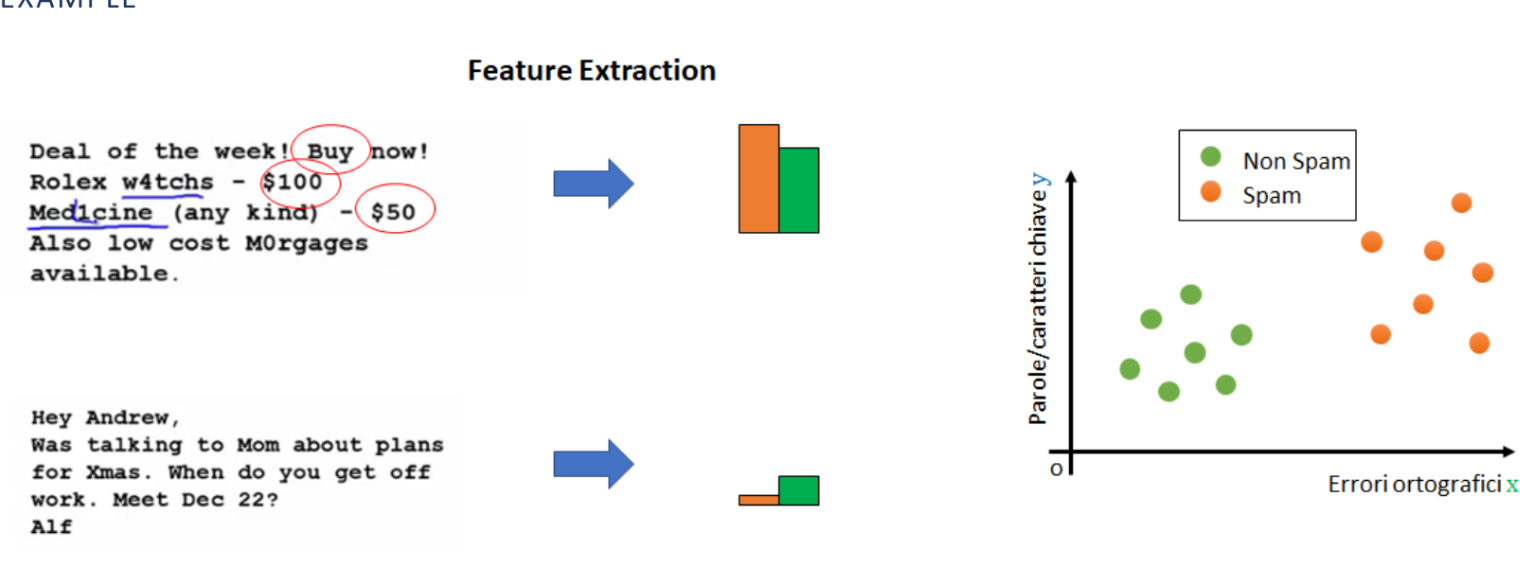
\includegraphics[width=\textwidth]{images/featureExtraction.png}
    \caption{Estrazione delle feature: le e-mail vengono trasformate in vettori 2D, dove $x_1 = \text{errori ortografici}$ e $x_2 = \text{pattern ripetibili}$, e proiettate nello spazio delle feature, dove la separazione tra spam (arancione) e non spam (verde) risulta evidente.}
    \label{fig:featureExtraction}
\end{figure}

\section{Tipologie di Task}

Le attivit\`a possono essere di diversi tipi. Di seguito, discuteremo due compiti principali:
\begin{itemize}
\item \textbf{Classificazione}.
\item \textbf{Regressione}.
\end{itemize}

Assumeremo che ogni algoritmo di apprendimento automatico prenda come input esempi che sono gi\`a stati rappresentati con una funzione di rappresentazione adeguata.

\subsection{Classificazione}

In questo tipo di attivit\`a, alla macchina viene chiesto di specificare a quale di un insieme predefinito di categorie $K$ appartiene l'input.

\noindent
Esempi di questo compito sono:
\begin{itemize}
\item Classificare i post di Facebook come riguardanti la politica o qualcos'altro (politica vs non politica).
\item Rilevamento delle e-mail di spam (spam vs e-mail legittime).
\item Riconoscimento dell'oggetto raffigurato in un'immagine tra 1000 oggetti diversi.
\end{itemize}

\noindent
L'algoritmo di apprendimento \`e solitamente fornito con un insieme di esempi:
\[
\{x^{(1)}, x^{(2)}, \dots, x^{(m)}\}
\quad \text{dove } x^{(i)} \in \mathbb{R}^{d}\ \forall i,
\]
e un insieme di etichette corrispondenti:
\[
\{y^{(1)}, y^{(2)}, \dots, y^{(m)}\}
\quad \text{dove } y^{(i)} \in \{1, \dots, K\}\ \forall i,
\]
che specificano a quale delle categorie $K$ appartiene ogni esempio. Ad esempio, se $y^{(i)} = 3$, allora $x^{(i)}$ appartiene alla classe ``3''.

Nel caso della classificazione binaria (ad esempio, spam vs non spam), $y^{(i)} \in \{0,1\}$. Per risolvere questo compito, l'algoritmo di apprendimento automatico assume la forma di una funzione:
\[
h_\theta: \mathbb{R}^{d} \rightarrow \{1, \dots, K\},
\]
tale che:
\[
y^{(i)} = h_\theta(x^{(i)}).
\]

\noindent
Esempio:
\begin{itemize}
    \item \textbf{Classification Task:} data un'e-mail, classificarla come spam o non spam.
    \item \textbf{Input:} esempi $d$-dimensionali $x=(x_1,\dots,x_d)$ contenenti le caratteristiche dell'e-mail.
    \item \textbf{Output:} etichette $y \in \{0,1\}$ che indicano se l'e-mail \`e legittima o spam.
\end{itemize}

Alcuni algoritmi di classificazione \textbf{non prevedono un output discreto}, ma un vettore di \textbf{probabilit\`a}, contenente la probabilit\`a relativa a ciascuna delle etichette possibili. In questo caso, puntiamo ad avere la probabilit\`a massima nello slot del vettore relativo all'etichetta vera.

\subsection{Regressione}

In questo tipo di compito, al programma del computer viene chiesto di \textbf{prevedere un valore numerico dato un input}, ad esempio:
\begin{itemize}
    \item Prevedere il prezzo delle case date alcune caratteristiche come la citt\`a, l'et\`a, la zona, ecc.
    \item Prevedere il valore futuro delle azioni di una societ\`a dai valori di altre societ\`a o da altre statistiche sul mercato.
    \item Contare il numero di auto presenti in un'immagine.
\end{itemize}

\noindent
Analogamente alla classificazione, l'algoritmo viene fornito con esempi di training $x \in \mathbb{R}^{d}$ e con gli output desiderati $y \in \mathbb{R}$. L'algoritmo di apprendimento automatico assume la forma di una funzione
\[
h_\theta: \mathbb{R}^{d} \rightarrow \mathbb{R}
\]
tale che $y^{(i)} = h_\theta(x^{(i)})$.

\noindent
Esempio:
\begin{itemize}
    \item \textbf{Regression task:} predire il prezzo di una casa in base ai suoi metri quadrati.
    \item \textbf{Input:} dimensione della casa $x$ (valore scalare).
    \item \textbf{Output:} prezzo $y$.
\end{itemize}

\noindent
Sono algoritmi ottimi per trovare relazioni tra i dati ed effettuare predizioni.

\begin{figure}[htp]
    \centering
    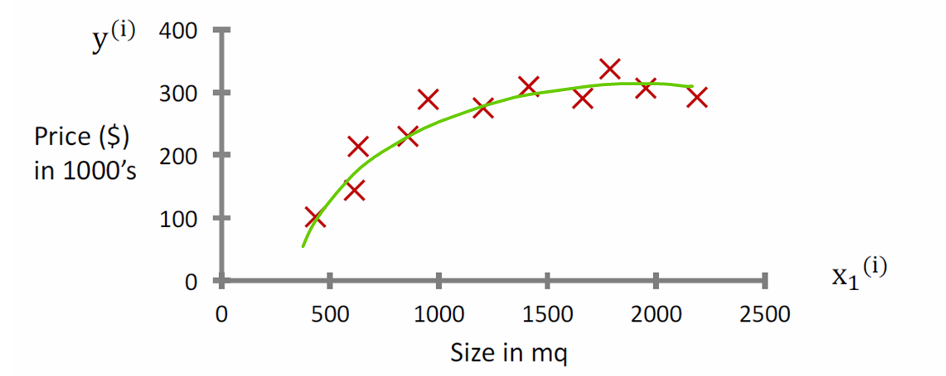
\includegraphics[width=\textwidth]{images/regression.png}
    \caption{Relazione tra dimensione dell'immobile $(x_1^{(i)}$, in mq) e prezzo $(y^{(i)}$, in migliaia di \$): i punti rossi sono i dati osservati, la linea blu rappresenta un modello di regressione lineare che non approssima bene l'andamento non lineare.}
    \label{fig:regressione}
\end{figure}

\section{Tipi di Machine Learning}

\subsection{Supervised Learning e Unsupervised Learning}

Gli approcci di Machine Learning possono essere approssimativamente divisi in \textbf{supervised} e \textbf{unsupervised learning}.

\paragraph{Supervised Learning:}
L'algoritmo viene addestrato su un insieme di esempi di input e \textbf{output desiderati}. L'obiettivo \`e allenare un modello a mappare gli input agli output corretti. Il punto chiave \`e conoscere gli output desiderati: i dati del dataset dovranno quindi essere preventivamente \textbf{etichettati}.

\paragraph{Unsupervised Learning:}
L'algoritmo viene addestrato solo su esempi di input, senza output desiderati. L'obiettivo \`e trovare struttura, pattern e associazioni nei dati, spesso molto eterogenei:
\[
\{x^{(1)}, x^{(2)}, \dots, x^{(m)}\}
\qquad \text{dove } x^{(i)} \in \mathbb{R}^{d}\ \forall i.
\]
Questi tipi di compiti mirano generalmente a \textbf{modellare la struttura dei dati}. Un esempio di unsupervised learning \`e il \textbf{clustering}, in cui non viene fornita alcuna informazione aggiuntiva oltre agli esempi.

Gli approcci supervised sono generalmente pi\`u facili da gestire, ma richiedono la presenza di \textbf{labels}. Ottenere labels \`e spesso un problema costoso in termini di tempo, poich\'e richiede che le persone annotino manualmente i dati. Ad esempio, se dobbiamo costruire uno spam-detector con un approccio supervised, \`e necessario che qualcuno etichetti manualmente diverse e-mail come ``spam'' o ``non-spam''.

\subsection{Reinforcement Learning}

Alcuni autori fanno riferimento anche a una terza classe di algoritmi di Machine Learning: il \textbf{Reinforcement Learning}.

Il Reinforcement Learning mira a \textbf{scoprire la soluzione a un problema} attraverso il metodo \emph{trial and error}, piuttosto che tramite istruzioni esplicite su come risolvere il compito. Questo avviene permettendo all'algoritmo di \textbf{interagire con un environment} e ricevere \textbf{positive rewards} quando compie azioni che portano a un buon risultato e \textbf{negative rewards} quando compie azioni che portano a un risultato negativo.

L'obiettivo degli algoritmi di Reinforcement Learning \`e apprendere una policy $\pi$, che possa essere utilizzata per \textbf{determinare quale azione intraprendere} quando si acquisisce un'\textbf{osservazione} del mondo $o$. Questo processo \textbf{ricorda il modo naturale in cui gli animali imparano a risolvere problemi}. Ad esempio, si pu\`o pensare a un topo che deve trovare l'uscita da un labirinto (immagine \ref{fig:reinforcementLearning}).

\begin{figure}[htp]
    \centering
    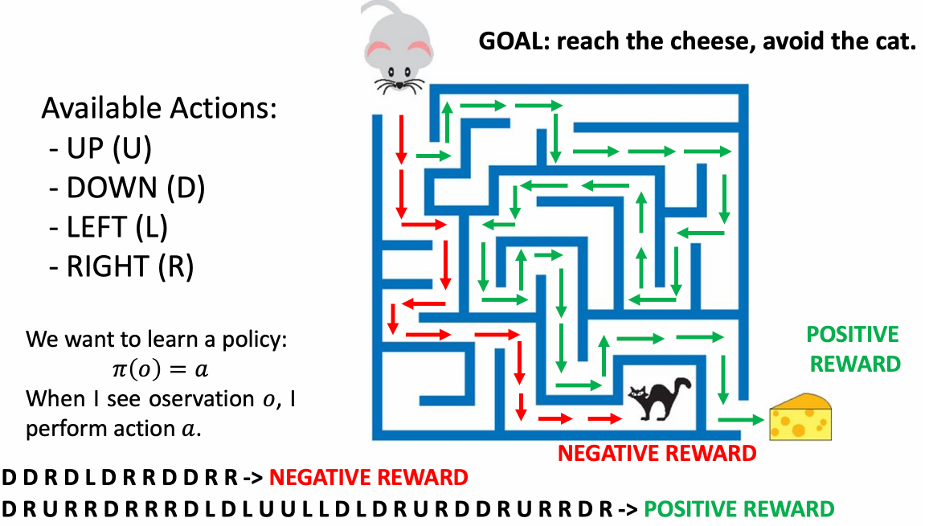
\includegraphics[width=\textwidth]{images/reinforcementLearning.png}
    \caption{Reinforcement Learning nel labirinto: l'agente sceglie tra azioni U/D/L/R e apprende una policy \(\pi(o)=a\) che massimizza la ricompensa, raggiungendo il formaggio (positiva) ed evitando il gatto (negativa).}
    \label{fig:reinforcementLearning}
\end{figure}

\section{Misura di Performance (P)}

Per valutare le capacit\`a di un algoritmo di Machine Learning nel risolvere un determinato compito, \`e necessaria una misura quantitativa delle sue prestazioni. Solitamente, questa \textbf{performance measure} $P$ \`e \textbf{specifica per il task} $T$ che il sistema sta eseguendo.

Per compiti come la classificazione, spesso si misura la performance utilizzando l'\textbf{accuracy}, ovvero la percentuale di esempi classificati correttamente dal modello. Nel caso della regressione, invece, si possono usare altre metriche come il mean squared error.

\noindent
Le misure di performance sono utilizzate per due motivi principali:
\begin{itemize}
\item Capire quando un algoritmo di Machine Learning sta migliorando in un determinato compito.
\item Valutare la performance dell'algoritmo una volta finalizzato.
\end{itemize}

\noindent
Quando $P$ \`e una metrica normalizzata (come l'accuracy), l'error rate si pu\`o calcolare come $1 - P$. Per metriche non normalizzate si usa una loss $\ell$.

\subsection{Esempio}

Un spam detector analizza cinque e-mail. Le prime tre sono spam, le ultime due non lo sono. L'algoritmo classifica come spam le prime due e-mail e come non spam le ultime tre. In questo caso, la prima e le ultime due classificazioni sono corrette, mentre la terza \`e errata. La accuracy si calcola come la percentuale di esempi classificati correttamente:
\[
\frac{4}{5} = 0.8 \quad \text{ovvero} \quad 80\%.
\]

\section{Elementi fondamentali del Machine Learning}

\subsection{Experience (E)}

Un algoritmo di Machine Learning apprende dall'\textbf{experience} per migliorare una performance measure su un determinato task.

\noindent
Nel supervised learning, l'experience coincide con un dataset $D$ di esempi osservati:
\[
D = \{(x^{(i)}, y^{(i)})\}_{i=1}^m,
\]
con $(x^{(i)}, y^{(i)})$ realizzazioni delle variabili aleatorie $(X,Y)$, spesso assunte i.i.d.\ secondo una distribuzione $\mathcal{D}$. Nel caso unsupervised, il dataset contiene solo gli input $\{x^{(i)}\}_{i=1}^m$.

\subsection{Dataset (D)}

Le performance measures vengono generalmente calcolate rispetto a un insieme di esempi, piuttosto che su singoli esempi. Un insieme di esempi (eventualmente con labels) \`e chiamato \textbf{dataset}. I dataset sono generalmente omogenei, nel senso che i dati contenuti al loro interno hanno un formato simile. Ad esempio:
\begin{itemize}
    \item Nel Fisher's Iris dataset, tutti gli esempi hanno 4 features e una label corrispondente a una delle tre classi.
    \item In un dataset di immagini di food, ogni immagine \`e associata a una classe che indica il piatto specifico.
\end{itemize}

\subsection{Design Matrix}

Un modo comune per rappresentare un dataset \`e utilizzare una design matrix. Poich\'e ogni esempio \`e una collezione di $d$ features, un dataset di $m$ elementi pu\`o essere rappresentato tramite una matrice:
\[
X \in \mathbb{R}^{m \times d}, \quad m,d \in \mathbb{N},
\]
di dimensione $m \times d$.

\begin{itemize}
    \item Ogni riga della design matrix rappresenta un esempio.
    \item Ogni colonna rappresenta una delle features.
\end{itemize}

\noindent
Nel caso del supervised learning, si considera spesso anche un vettore di etichette:
\[
Y \in \{1, \dots, K\}^{m},
\]
dove $K$ \`e il numero di classi (nel caso di classificazione). Nel caso di regressione, invece, $Y \in \mathbb{R}^m$.

\begin{figure}[htbp]
    \centering
    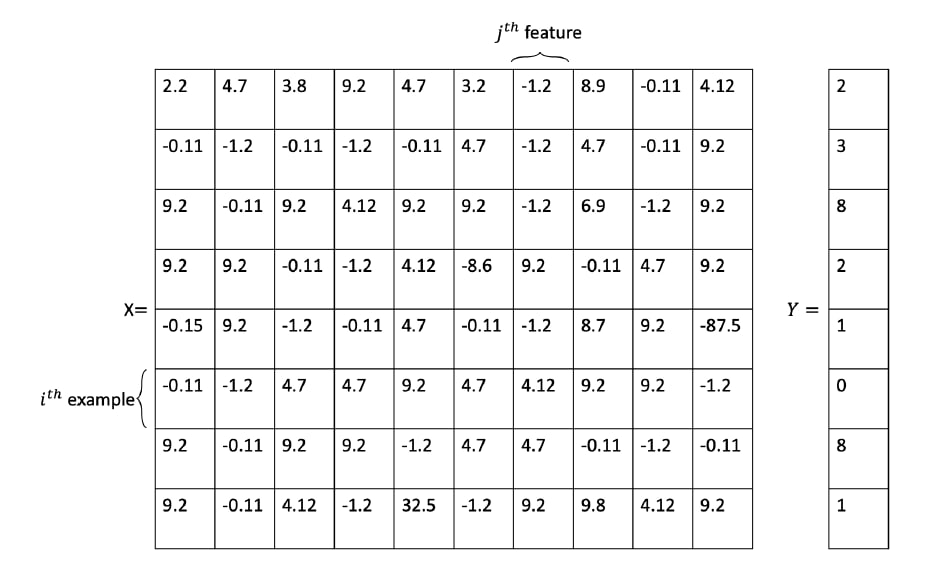
\includegraphics[width=\textwidth]{images/designMatrix.jpg}
    \caption{Design Matrix: rappresentazione di un dataset con $m$ esempi e $d$ features. Ogni riga corrisponde a un esempio, ogni colonna a una feature.}
    \label{fig:designMatrix}
\end{figure}

\subsection{Esempio}

Supponiamo di avere un dataset composto da 1000 e-mail, alcune classificate come spam e altre come not spam. Assumiamo che ogni e-mail sia rappresentata da due features, come discusso nei precedenti esempi.

\noindent
La design matrix che rappresenta il dataset \`e una matrice:
\[
X \in \mathbb{R}^{1000 \times 2}.
\]

\begin{itemize}
\item Ogni elemento della matrice rappresenta una delle features di un esempio nel dataset.
\item Ad esempio, $X_{i,1}$ indica il numero di \textbf{errori} ortografici nell'$i$-\textbf{esima} e-mail, mentre $X_{i,2}$ rappresenta il numero di \textbf{occorrenze} di parole chiave nella stessa e-mail.
\end{itemize}

\noindent
Le labels sono contenute in un vettore:
\[
Y \in \{0,1\}^{1000},
\]
dove $Y_i$ rappresenta la label associata all'$i$-\textbf{esimo} esempio (ad esempio, 0 = not spam, 1 = spam).

\subsection{Learning}

Un algoritmo di Machine Learning \textbf{utilizza un dataset di esempi} per \textbf{migliorare la sua performance} in un determinato \textbf{task}. Il processo di miglioramento della performance dell'algoritmo \`e chiamato \textbf{learning} o \textbf{training}.

\paragraph{In cosa consiste il training?}

\begin{itemize}
\item Un algoritmo di Machine Learning ha alcuni parametri (parameters), che possono essere regolati per modificarne il comportamento. Questi parametri sono legati a un model (una funzione matematica) utilizzata per risolvere il task.
\item Un algoritmo chiamato training procedure utilizza gli esempi forniti per trovare i valori ottimali per questi parameters.
\item Alcuni parametri non possono essere regolati automaticamente dal training. Questi sono detti hyperparameters e devono essere ottimizzati al di fuori della training procedure, spesso attraverso un metodo trial and error.
\end{itemize}

\paragraph{Esempio.}

Consideriamo un semplice spam detector che classifica le e-mail come spam o non-spam in base al numero di errori ortografici.

\noindent
L'algoritmo pu\`o essere scritto come segue:

\begin{lstlisting}[style=py,caption={Soglia sul numero di errori ortografici, chiaramente un approccio naive},label={lst:spam-threshold}]
def classify(x):
    if x > a:
        return 1  # Spam
    else:
        return 0  # Non-spam
\end{lstlisting}

\noindent
L'algoritmo dipende da un singolo parametro $a$. La domanda \`e: quale valore dovremmo assegnare ad $a$? La \emph{training procedure} permette di trovare un valore ottimo presumibilmente adatto per $a$.

\noindent
Una semplice training procedure consisterebbe nel provare diversi valori per $a$ e registrare le performance dell'algoritmo per ciascun valore di $a$. Alla fine, possiamo scegliere il valore di $a$ che massimizza la performance measure $P$ (o, in alternativa, minimizza una loss $\ell$).

\subsection{Rischio atteso e rischio empirico}

Per formalizzare l'idea di ``buone prestazioni'' si introduce una loss $\ell$ e si definisce il \textbf{rischio atteso} (o \emph{true risk}):
\[
R(\theta) = \mathbb{E}_{(x,y)\sim \mathcal{D}}\bigl[\ell(h_\theta(x), y)\bigr].
\]

\noindent
Poich\'e la distribuzione $\mathcal{D}$ \`e sconosciuta, in pratica si minimizza il \textbf{rischio empirico} sul dataset osservato $D$:
\[
\hat{R}(\theta) = \frac{1}{m}\sum_{i=1}^m \ell\bigl(h_\theta(x^{(i)}), y^{(i)}\bigr).
\]

\noindent
La differenza $R(\theta) - \hat{R}(\theta)$ \`e detta \textbf{generalization gap}: minimizzare $\hat{R}$ non garantisce necessariamente di minimizzare $R$, specialmente con modelli molto complessi (overfitting). Per questo si valutano le prestazioni su dati non visti (testing) e si usano strategie come la cross-validation per stimare la capacit\`a di generalizzazione.

\subsection{Il paradigma Training/Testing}

Ciascun algoritmo di Machine Learning presenta al suo interno dei parametri. Una scelta opportuna dei parametri dovrebbe garantire il funzionamento del modello. La procedura generale per la scelta e la verifica dei parametri dell'algoritmo \`e suddivisa in due parti:

\begin{enumerate}
\item \textbf{Training dell'algoritmo}.\\
Effettuato usando i dati del \textbf{training set}, consiste nella scelta dei parametri del modello, osservando i valori della \textit{loss function} (o funzione di costo), che offre un indice dell'errore da parte del modello e permette di capire se i parametri vanno modificati, e di quanto.
\item \textbf{Testing dell'algoritmo - Inferenza}.\\
Si passa poi ai dati di testing, usati per verificare se i parametri scelti sul dataset di training sono opportuni su dati mai visti prima. Il modello viene quindi valutato secondo le \textbf{misure di valutazione}.
\end{enumerate}

\subsubsection*{Suddivisione dei dati}

Distinguiamo due insiemi di dati: i \textbf{dati di training} e i \textbf{dati di testing}. \`E importante che i dati usati in fase di training e i dati usati in fase di inferenza siano \textbf{totalmente disgiunti}:
\[
D_{\text{train}} \cap D_{\text{test}} = \varnothing.
\]

Tuttavia, entrambi i set di dati appartengono in origine allo stesso dataset $D$. La suddivisione dei dati in training e testing sar\`a effettuata randomicamente, in modo da evitare bias di qualsiasi tipo. Dobbiamo inoltre assicurarci che il numero di dati, per ogni etichetta, sia bilanciato. Prendere l'80\% di un dataset in fase di testing, con due classi (cane, non-cane), significa prendere l'80\% di ciascuna delle due classi. L'obiettivo \`e \textbf{evitare favoritismi} durante la classificazione. Parleremo pi\`u avanti di tecniche che stabiliscono come effettuare la suddivisione tra training e testing sfruttando al meglio i propri dati, come la $k$-fold cross-validation.

\subsection{Normalizzazione}

I nostri dati $x \in \mathbb{R}^d$ possono avere valori appartenenti a range molto ampi, con scale diverse per ciascuna feature. Per creare spazi in cui le features hanno pi\`u o meno la stessa scala, si usano strategie di normalizzazione, come di seguito.

\paragraph{Normalizzazione in $[0,1]$.}
Per ogni $j$-esima feature, dobbiamo stabilire il minimo e il massimo del dataset. Dato un dataset di dimensione $m$:
\begin{align*}
  x_j^{\min } &= \min\{x_j^{(i)} \mid i = 1, 2, \dots, m\},\\
  x_j^{\max } &= \max\{x_j^{(i)} \mid i = 1, 2, \dots, m\}.
\end{align*}
Possiamo quindi normalizzare secondo la seguente formula:
\[
  \hat{x}_j = \frac{x_j - x_j^{\min}}{x_j^{\max} - x_j^{\min}},
\]
e ogni dato sar\`a $\hat{x}_j \in [0,1]$.

\paragraph{Standardizzazione in $[-1,1]$.}
\[
  \hat{x}_j = \frac{x_j - \mu_j}{\sigma_j}
\]
con $\sigma_j$ deviazione standard (la varianza \`e $\sigma_j^2$). Il risultato \`e un centramento rispetto alla media: l'origine coincide con la media, e i dati risultano su una scala comparabile.

\subsubsection*{Quantit\`a statistiche per la $j$-esima feature}

Per completezza, riportiamo le definizioni delle quantit\`a usate sopra:
\begin{align*}
  \text{Media:}\quad
  \mu_j &= \frac{1}{m}\sum_{i=1}^m x_j^{(i)},\\[4pt]
  \text{Varianza:}\quad
  \mathrm{Var}(x_j) &= \frac{1}{m}\sum_{i=1}^m \bigl(x_j^{(i)}-\mu_j\bigr)^2,\\[4pt]
  \text{Deviazione standard:}\quad
  \sigma_j &= \sqrt{\frac{1}{m}\sum_{i=1}^m \bigl(x_j^{(i)}-\mu_j\bigr)^2}
           \;=\; \sqrt{\mathrm{Var}(x_j)}.
\end{align*}

Bisogner\`a conservare rispettivamente $x_j^{\min }, x_j^{\max }$ oppure $\mu_j, \sigma_j$, per permettere la normalizzazione del testing set, in quanto la normalizzazione \`e fatta in fase di training.

\section{Iperparametri}

Sono parametri che stabiliscono aspetti del modello e che non sono calcolati in fase di training. In fase di training, questi vengono fissati e \textbf{non vengono stimati} dalla training procedure. Nonostante ci\`o, gli iperparametri hanno un effetto sulla loss function e quindi sulle prestazioni finali. Bisogner\`a variare gli iperparametri usando un \textbf{validation set}, un terzo set di dati ottenuto dal dataset $D$.

\subsection{k-fold Cross Validation}

\`E una strategia che permette di ottenere buoni risultati anche con dataset pi\`u piccoli. Dividiamo in due parti il dataset $D$, ottenendo l'insieme di training e l'insieme di testing. Dividiamo nuovamente l'insieme di \textbf{training} in $k$ parti. Supponiamo $k=3$: utilizzeremo una porzione $\frac{1}{k}$ per la validazione e le $\frac{k-1}{k}$ rimanenti come training. In questo caso, $1/3$ e $2/3$. Effettueremo quindi tre cicli di training e validazione, variando ogni volta il subset usato per la validazione. Da ciascuno dei processi di training emerger\`a un valore della loss function: sceglieremo gli iperparametri associati a valori della loss pi\`u bassi (o, in alternativa, a metriche di performance pi\`u alte).

\begin{figure}[htbp]
\centering
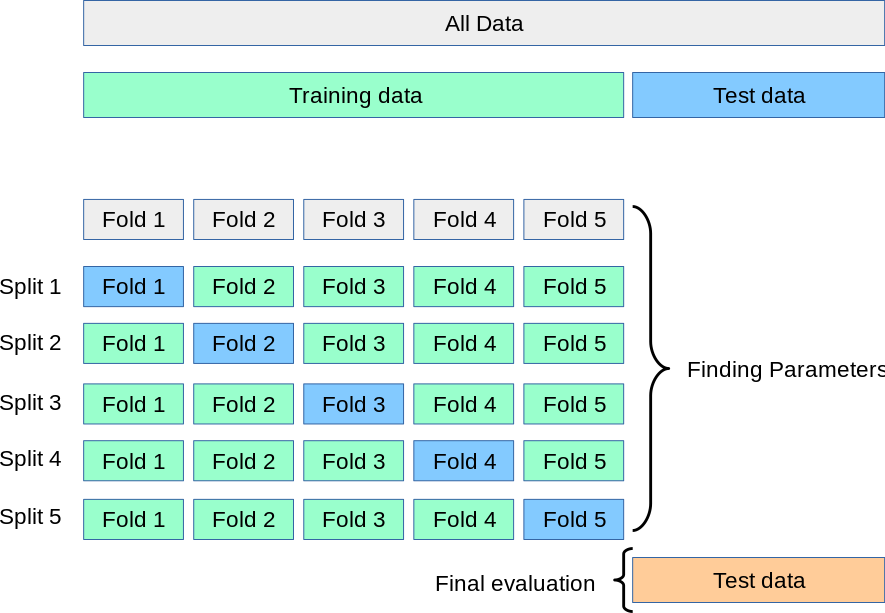
\includegraphics[width=0.8\textwidth]{images/cross_validation.png}
\caption{Procedura di cross-validation con $k=5$.}
\label{fig:crossValidation}
\end{figure}

\section{Overfitting e underfitting}

Sono tra i problemi pi\`u grandi che possono emergere con i propri algoritmi di machine learning e riguardano spesso la \textbf{scelta del modello}.

\begin{description}
    \item[Overfitting] Si parla di overfitting quando il modello \`e cos\`\i\ complesso da offrire performance ottime in fase di training, ma fortemente \textbf{peggiori in fase di testing}: il modello ha imparato troppo bene (anche dettagli e rumore) i dati su cui ha appreso, ma generalizza male sui dati inediti.
    \item[Underfitting] \`E caratterizzato da \textbf{pessime performance in fase di training}: troppe poche variabili o modello troppo semplice. L'apprendimento non \`e tale da permettere al modello di catturare la struttura dei dati. Il modello non impara.
\end{description}

Bisogna quindi trovare lo \textit{sweet spot}, il compromesso tra modelli pi\`u complessi e modelli pi\`u semplici. Il numero di parametri \`e un fattore da tenere sempre in considerazione.

\subsection{Bias e Variance}

\begin{figure}[htbp]
\centering
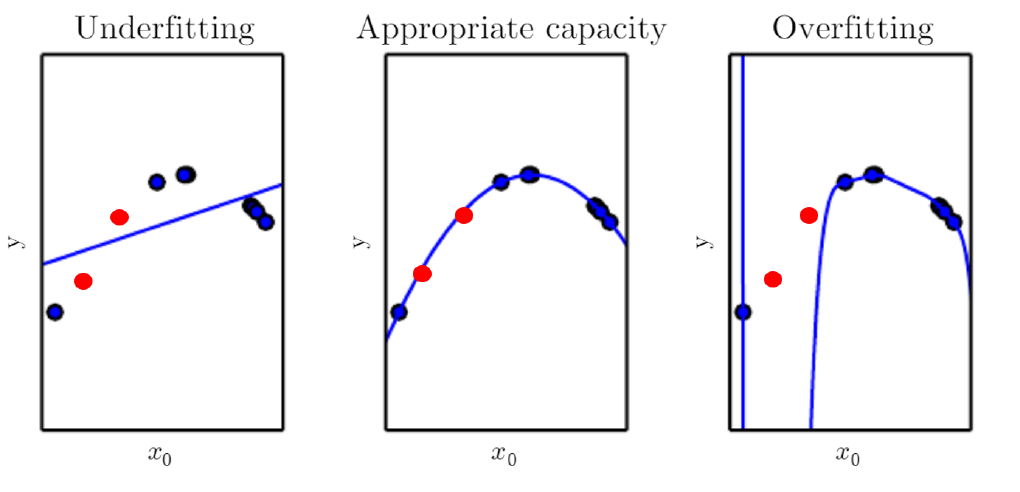
\includegraphics[width=0.6\textwidth]{images/underoverfitting}
\caption{In blu i dati di training, in rosso quelli di testing. Nel caso dell'underfitting, vediamo una funzione troppo semplice (una funzione lineare) per approssimare una funzione pi\`u complessa. Nel caso dell'overfitting, il modello d\`a output assurdi.}
\label{fig:underoverfitting}
\end{figure}

\noindent
Osservando i risultati dei nostri modelli, \`e possibile individuare facilmente due tipologie di errori:

\begin{description}
    \item[Bias Error.] Le previsioni non sono corrette a causa di assunzioni errate nel modello. Un alto bias pu\`o portare il modello a non rilevare importanti relazioni tra le features e gli output target, portando a underfitting (es.\ un modello che cerca di approssimare una funzione polinomiale con una lineare).
    \item[Variance Error.] Le previsioni del modello sono fortemente influenzate da piccole fluttuazioni nel training set. Ad esempio, se rimuoviamo un punto dati e riaddestriamo l'algoritmo, otteniamo previsioni molto diverse. Questo pu\`o essere dovuto al fatto che l'algoritmo sta cercando di modellare il rumore casuale presente nei dati di training, il che di solito porta a overfitting.
\end{description}

\noindent
La \textbf{decomposizione bias-varianza} si riferisce tipicamente all'\textbf{errore atteso} (ad esempio per la MSE) e non va confusa con la differenza tra errori di training e testing.

\section*{Riferimenti}

Il materiale visto in questo capitolo comprende:
\begin{itemize}
    \item Materiale visto a lezione.
    \item Note scritte dal prof.\ Antonino Furnari.
\end{itemize}
